\section{系统框架与模块实现}
\label{sec-2}
\subsection{整体框架}
\begin{frame}[label=sec-2-1]{整体框架}
  \transdissolve<2->
  \centering
  \vspace{-2mm}
  \begin{tikzpicture}[scale=.57,transform shape,
    font=\large,
    io/.style={fill=black!30, text width=3cm, minimum size=1cm,align=center,draw=black},
    submodule/.style={fill=cyan!80, text width=3cm, minimum size=1cm, rounded corners,align=center,draw=black},
    bold arrow/.style={very thick, >=triangle 90}
    ]    
    \node (input) [io] {输入网页};
    \visible<2->{\node (input-arrow) [below=1mm of input]
    [single arrow, minimum width=5mm, minimum height=0.8cm, shape border rotate=270, draw]{};}
    \node (m1-1) [submodule, below=4mm of input-arrow]{过滤无用网页};
    \node (m1-2) [submodule, below=5mm of m1-1]{简化HTML文档} edge[<-] (m1-1);
    \node (m2-1) [submodule, below=1.2cm of m1-2]{结构相似度计算};
    \visible<4->{\draw [<-, bold arrow] (m2-1) -- (m1-2);}
    \node (m2-2) [submodule, below=5mm of m2-1]{网页聚类} edge[<-] (m2-1);
    \node (m3-1) [submodule, below=1.2cm of m2-2]{模板生成};
    \visible<6->{\draw [<-, bold arrow] (m3-1) -- (m2-2);}
    \node (m3-2) [submodule, below=5mm of m3-1]{内容抽取} edge[<-] (m3-1);
    \node (new-input) [io, left=of m3-2]{新的网页输入};
    \node (output) [io, below=of m3-2]{XML输出};
    \visible<8->{\draw [->, bold arrow] (new-input) -- (m3-2);
    \draw [<-, bold arrow] (output) -- (m3-2);}
  \begin{pgfonlayer}{background}
    \tikzset{module/.style={inner sep=1em, fill=white, dashed, draw=black, rounded corners}};
    \visible<3->{\node (m1)[module, fit=(m1-1) (m1-2)]{};
    \invisible<9>{\node (m1-name) [right=5mm of m1]{\Large{预处理模块}};}}
    \visible<5->{\node (m2)[module, fit=(m2-1) (m2-2)]{} [below=of m1];
    \invisible<9>{\node (m2-name) [right=5mm of m2]{\Large{网页聚类模块}};}}
    \visible<7->{\node (m3)[module, fit=(m3-1) (m3-2)]{} [below=of m2];
    \invisible<9>{\node (m37name) [right=5mm of m3] {\Large{模板生成和内容提取模块}};}}
    \visible<9>{
      \node (offline) [draw, inner sep=3mm, fill=orange!20, fit=(input) (m1-1) (m1-2) (m2-1) (m2-2) (m3-1)]
      [label={[red]right:\LARGE{离线处理部分}}]{};}
    \visible<10>{
      \node (online) [draw, inner sep=3mm, fill=green!30,fit=(m3-2) (new-input) (output), rounded corners]
      [label={[red]right:\LARGE{在线处理部分}}]{};}
  \end{pgfonlayer}  
\end{tikzpicture}
\end{frame}
\subsection{预处理模块}
\begin{frame}{预处理模块介绍}
  \transdissolve<2->
  \centering
  \vspace{-2mm}
  \begin{tikzpicture}[scale=.58,transform shape,
    font=\large,
    io/.style={fill=black!30, text width=3cm, minimum size=1cm,align=center,draw=black},
    submodule/.style={fill=cyan!80, text width=3cm, minimum size=1cm, rounded corners,align=center,draw=black},
    bold arrow/.style={very thick, >=triangle 90},
    mylabel/.style={dotted, draw}
    ]    
    \node (input) [io] {输入网页};
    \visible<2->{\node (input-arrow) [below=1mm of input]
    [single arrow, minimum width=5mm, minimum height=0.8cm, shape border rotate=270, draw]{};}
  \visible<4->{
    \node (m1-1) [submodule, below=4mm of input-arrow]{过滤无用网页};}
  \invisible<1->{
    \node (m1-2) [submodule, below=5mm of m1-1]{简化HTML文档} edge[<-] (m1-1);
    \node (m2-1) [submodule, below=1.2cm of m1-2]{结构相似度计算};
    \draw [<-, bold arrow] (m2-1) -- (m1-2);
    \node (m2-2) [submodule, below=5mm of m2-1]{网页聚类} edge[<-] (m2-1);
    \node (m3-1) [submodule, below=1.2cm of m2-2]{模板生成};
    \draw [<-, bold arrow] (m3-1) -- (m2-2);
    \node (m3-2) [submodule, below=5mm of m3-1]{内容抽取} edge[<-] (m3-1);
    \node (new-input) [io, left=of m3-2]{新的网页输入};
    \node (output) [io, below=of m3-2]{XML输出};
    \draw [->, bold arrow] (new-input) -- (m3-2);
    \draw [<-, bold arrow] (output) -- (m3-2);
    }
  \begin{pgfonlayer}{background}
    \tikzset{module/.style={inner sep=1em, fill=white, dashed, draw=black, rounded corners}};
    \visible<3->{\node (m1)[module, fit=(m1-1) (m1-2)]{};
    \node (m1-name) [right=5mm of m1]{\Large{预处理模块}};}
  \invisible<1->{
    \node (m2)[module, fit=(m2-1) (m2-2)]{} [below=of m1];
    \node (m2-name) [right=5mm of m2]{\Large{网页聚类模块}};
    \node (m3)[module, fit=(m3-1) (m3-2)]{} [below=of m2];
    \node (m37name) [right=5mm of m3] {\Large{模板生成和内容提取模块}};
  }
      \invisible<1->{
      \node (offline) [draw, inner sep=3mm, fill=orange!20, fit=(input) (m1-1) (m1-2) (m2-1) (m2-2) (m3-1)]
      [label={[red]right:\LARGE{离线处理部分}}]{};
      \node (online) [draw, inner sep=3mm, fill=green!30,fit=(m3-2) (new-input) (output), rounded corners]
      [label={[red]right:\LARGE{在线处理部分}}]{};}
  \end{pgfonlayer}  
\end{tikzpicture}
\end{frame}

\begin{frame}[fragile,label=sec-2-2]{预处理模块-过滤无用网页}
  \transdissolve<3,5>
  \begin{block}{错误页过滤}
    \begin{itemize}
    \item<2->  404等错误页大小一般比较小
    \item<3->  方法:通过设置文件大小阈值过滤
    \end{itemize}
  \end{block}
  \begin{block}{目录页过滤}
  \begin{itemize}[<+->]
  \item<4-> 目录页的URL有一定的模式:比如对于新浪博客来说,详细页的 URL 都以.html 结尾,而
    目录页则没有。以下两个URL: \scriptsize
\begin{verbatim}
http://blog.sina.com.cn/u/1439351555
http://blog.sina.com.cn/s/blog_55cac30301016yb1.html
\end{verbatim}
     \normalsize
     第一个URL对应的是某个博主的文章目录,第二个URL则是该博主的某篇文章。
   \item<5-> 方法:通过为每类网页分别建立正则表达式的方法过滤目录页
    \end{itemize}     
 \end{block}
\end{frame}

\begin{frame}[label=sec-2-3]{预处理模块-过滤无用网页}  
  \begin{block}{目录页过滤}
    \begin{itemize}
    \item 为了完备性考虑,可能存在某些网站,目录页的 URL 和详细页的 URL 在模式没有
      太大的区别,或者人工设置规则的办法太麻烦了
     \item<2-> 观察百度新闻目录页部分简化的HTML代码:
       \begin{figure}[h]
        \centering
        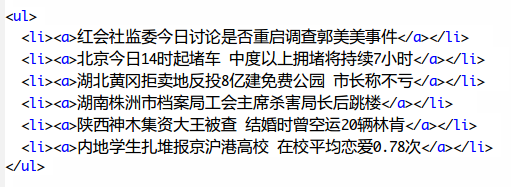
\includegraphics[width=0.6\textwidth]{baidunews}
      \end{figure}    
    \item<3-> 我们提取出网页中的所有<li>标签中的<a>标签,计算这些<a>标签的文本内容
      占网页所有文本内容的比重,超过一定的阈值则判定为目录页。
    \end{itemize}
\end{block}
\end{frame}
\begin{frame}{预处理模块介绍}
  \transdissolve<2->
  \begin{tikzpicture}[scale=.58,transform shape,
    font=\large,
    io/.style={fill=black!30, text width=3cm, minimum size=1cm,align=center,draw=black},
    submodule/.style={fill=cyan!80, text width=3cm, minimum size=1cm, rounded corners,align=center,draw=black},
    bold arrow/.style={very thick, >=triangle 90},
    mylabel/.style={dotted, draw}
    ]    
    \node (input) [io] {输入网页};
    \node (input-arrow) [below=1mm of input]
    [single arrow, minimum width=5mm, minimum height=0.8cm, shape border rotate=270, draw]{};
      \node (m1-1) [submodule, below=4mm of input-arrow]{过滤无用网页};
      \visible<2->{\node (m1-2) [submodule, below=5mm of m1-1]{简化HTML文档} edge[<-] (m1-1);}
  \invisible<1->{
  \node (m2-1) [submodule, below=1.2cm of m1-2]{结构相似度计算};
    \draw [<-, bold arrow] (m2-1) -- (m1-2);
    \node (m2-2) [submodule, below=5mm of m2-1]{网页聚类} edge[<-] (m2-1);
    \node (m3-1) [submodule, below=1.2cm of m2-2]{模板生成};
    \draw [<-, bold arrow] (m3-1) -- (m2-2);
    \node (m3-2) [submodule, below=5mm of m3-1]{内容抽取} edge[<-] (m3-1);
    \node (new-input) [io, left=of m3-2]{新的网页输入};
    \node (output) [io, below=of m3-2]{XML输出};
    \draw [->, bold arrow] (new-input) -- (m3-2);
    \draw [<-, bold arrow] (output) -- (m3-2);
    }
  \begin{pgfonlayer}{background}
    \tikzset{module/.style={inner sep=1em, fill=white, dashed, draw=black, rounded corners}};
    \node (m1)[module, fit=(m1-1) (m1-2)]{};
    \node (m1-name) [right=5mm of m1]{\Large{预处理模块}};
  \invisible<1->{
    \node (m2)[module, fit=(m2-1) (m2-2)]{} [below=of m1];
    \node (m2-name) [right=5mm of m2]{\Large{网页聚类模块}};
    \node (m3)[module, fit=(m3-1) (m3-2)]{} [below=of m2];
    \node (m37name) [right=5mm of m3] {\Large{模板生成和内容提取模块}};
  }
      \invisible<1->{
      \node (offline) [draw, inner sep=3mm, fill=orange!20, fit=(input) (m1-1) (m1-2) (m2-1) (m2-2) (m3-1)]
      [label={[red]right:\LARGE{离线处理部分}}]{};
      \node (online) [draw, inner sep=3mm, fill=green!30,fit=(m3-2) (new-input) (output), rounded corners]
      [label={[red]right:\LARGE{在线处理部分}}]{};}
  \end{pgfonlayer}  
\end{tikzpicture}
\end{frame}

\begin{frame}[t,label=sec-2-4]{预处理模块-简化HTML文档}
  \transdissolve<4>
  \begin{block}{简化HTML文档的3个步骤}
\begin{enumerate}
\item 去除无用标签。<script>、<link>、<style>、 <br/>等。
\item<2-> 简化解析好的DOM Tree树形结构: 采用先序遍历的方式,将DOM Tree 转化成一个标签
  序列。
  \begin{tikzpicture}
  \node (dom) {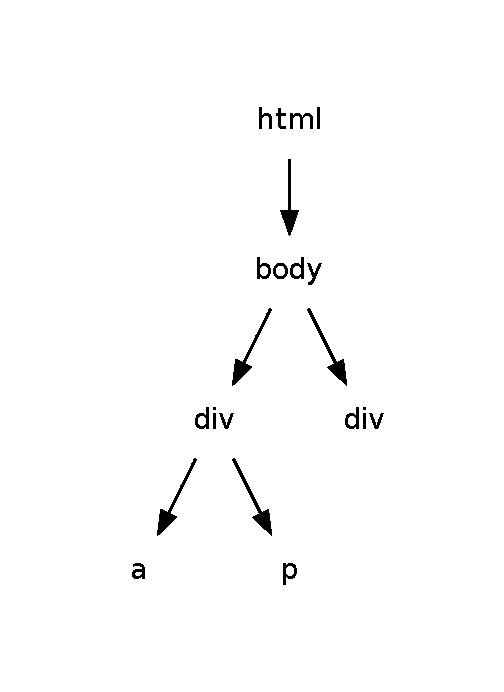
\includegraphics[width=0.3\textwidth]{domtree}};
  \visible<3->{\node (arrow) [fill=cyan!50, right=of dom, draw, single arrow, minimum height=1cm, minimum width=5mm] {};
  \node (seq) [right=of arrow,align=left]
  {\small <html0><body1>\\
    <div2><a3><p3>\\
    <div2>};}
  \end{tikzpicture}
  \vspace{-1cm}
\item<4-> \alert<5>{利用后缀树检测并合并重复记录}
\end{enumerate}
\end{block}
\end{frame}

\begin{frame}[label=sec-2-6]{检测重复记录}
  \begin{block}{动机}
    \begin{itemize}
    \item 网页模板中有大量不定个数的重复模式,通常由模板语言的for语句生成,我们需
      要将这些记录合并
    \end{itemize}    
    \begin{figure}[h]
      \centering
      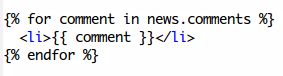
\includegraphics[width=0.4\textwidth]{django-for}
    \end{figure}
  \end{block}
  \pause
  \begin{block}{后缀树简介}
\begin{itemize}
\item 一种可以快速完成重复字串的查找的数据结构。
\item 定义:由序列所有的后缀组成的Trie树。
\item 后缀树普通的构造算法复杂度很高,系统实现中采用了Ukkonen在1995年提出了一个
  \(O(n)\)时间复杂度的在线构造算法。
\end{itemize}
  \end{block}
\end{frame}

\begin{frame}[label=sec-2-7]{后缀树示例}
BANANA对应的的后缀树
\begin{figure}[hb]
\centering
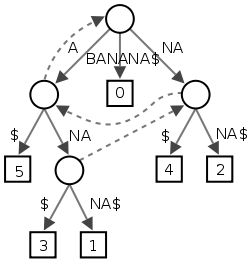
\includegraphics[width=0.5\textwidth]{./suffix-tree-banana.png}
\end{figure}
\end{frame}

\begin{frame}[label=sec-2-8]{后缀树查找重复序列算法}
\begin{block}{原始算法}
\begin{itemize}
\item 任意一条从根节点到内部节点的路径组成的序列都是原序列中重复出现的字串,且重复的次
数是以该内部节点为根的子树的叶子节点个数。
\item 缺点:没有考虑结构信息,从串映射回树结构时不一定符合要求。
\end{itemize}
\end{block}
\pause
\begin{block}{错误情况举例}
  \begin{itemize}[<+->]
\item \texttt{\small <div4><a5><div3><div4><a5><div3>}中的重复串\texttt{\small <div4><a5><div3>}横跨了两个不同子树。
\item \texttt{\small <div3><div4><a5><p5><div3><p4><a5><p5>}中的两个重复串\texttt{\small <a5><p5>}分属不同的子树。
\item \texttt{\small <div3><div4><div3><div4><a5><p5><div4><a5><p5>}中的重复串\texttt{\small <div3><div4>}和\texttt{\small <div4><a5><p5>}有交集\texttt{\small <div4>}。
  \end{itemize}
\end{block}
\end{frame}
\begin{frame} {新的算法要求}
\begin{itemize}
\item 重复序列不能横跨两个子树
\item 重复序列必须有公共的父亲
\item 不同的重复序列不能相交,不能互相包含
\item 重复序列必须尽可能地长
\end{itemize}
\end{frame}

\begin{frame}{后缀树查找重复序列算法-1}
  特点1:\alert<2->{保证序列尽可能长}
  \visible<2->{
\begin{block}{}
\begin{algorithm}[H]
  \caption{从根节点出发,找出所有的重复子序列\label{suffixtree:algo:fromroot}}
  \begin{algorithmic}[1]
    \Require 已经构建好的后缀树,根为$root$
    \Ensure 该后缀树中所有的重复子序列
    \State $//$从根节点出发,寻找所有的重复子序列
    \For{$edge \gets root.edges~\mathbf{if}~edge.endNode.isNotLeaf$}
    \State $//$取后缀树根节点的每条边的第一个元素作为每个子树的根节点
    \State $subTreeRoot := edge.firstElement$
    \State $//$查找以该节点为根的所有重复子序列
    \State findAllRepetitions$(root, \mathbf{nil}, subTreeRoot)$
    \EndFor
  \end{algorithmic}
\end{algorithm}
\end{block}
}
\end{frame}

\begin{frame}{后缀树查找重复序列算法-2}
   特点2:\alert<2->{保证序列不会横跨多个子树,且不互相包含}
   \visible<2->{
  \begin{block}{}
\floatname{algorithm}{\tiny 算法}
  \begin{algorithm}[H]
  \caption{\tiny 简化的findAllRepetitions实现}
  \label{suffixtree:algo:findrep}
  \begin{algorithmic}
    \tiny
    \Require 一个内部节点$node$,当前已经找到的重复序列$prefix$,要找的
    子树的根节点$subTreeRoot$
    \Ensure 所有经过该内部节点的符合要求的重复序列
    \Function {findAllRepetitions}{$node, prefix, subTreeRoot$}
    \State $//$定义一个空集合
    \State $results := Collection.empty$
    \State $//$对于该内部节点的每一条不连接叶子节点的边
    \For{$edge \gets node.edges~\mathbf{if}~edge.endNode.isNotLeaf$}
    \State $//$依次取出该条边上属于该根节点子树上的点
    \State $seq := edge.takeWhile(element$ inSubTreeOf $subTreeRoot)$\label{suffixtree:code:equals}
    \If {$seq.length == edge.length$}
    \State $//$遍历完了该条边上所有元素,
    \State $//$则取该条边连接的下一个内部节点进行递归查找
    \State findAllRepetitions($edge.endNode, prefix + seq, subTreeRoot$)
    \Else
    \State $//$否则,将当前得到的序列加入到结果集合中
    \State addToResults$(prefix + seq, results)$\label{suffixtree:code:add}
    \EndIf
    \EndFor
    \State \Return{$results$}
    \EndFunction
    \State
  \end{algorithmic}
\end{algorithm}
\end{block}
}
\end{frame}

\begin{frame}{后缀树查找重复序列算法-3}
  \vspace{-2.5cm}
  特点3:\alert<2->{保证重复序列相交均在同一子树中,且无相交的情况}
  \vspace{5mm}
  \visible<2->{
\begin{itemize}
\item 所有序列按实际的父节点分组,然后对每个分组进行合并,保证重复串有公共的父亲。
\item 对于重复串存在交集的情况,如之前的例子:
\texttt{\small <div3><div4><div3><div4><a5><p5><div4><a5><p5>}

对于\texttt{\small <div3><div4>} 和 \texttt{\small <div4><a5><p5>},只取 \texttt{<div4><a5><p5>}
\end{itemize}
}
\end{frame}

\subsection{网页聚类模块}
\begin{frame}{网页聚类模块介绍}
  \transdissolve<2->
  \begin{tikzpicture}[scale=.58,transform shape,
    font=\large,
    io/.style={fill=black!30, text width=3cm, minimum size=1cm,align=center,draw=black},
    submodule/.style={fill=cyan!80, text width=3cm, minimum size=1cm, rounded corners,align=center,draw=black},
    bold arrow/.style={very thick, >=triangle 90},
    mylabel/.style={dotted, draw}
    ]    
    \node (input) [io] {输入网页};
    \node (input-arrow) [below=1mm of input]
    [single arrow, minimum width=5mm, minimum height=0.8cm, shape border rotate=270, draw]{};
      \node (m1-1) [submodule, below=4mm of input-arrow]{过滤无用网页};
      \node (m1-2) [submodule, below=5mm of m1-1]{简化HTML文档} edge[<-] (m1-1);
  \visible<4->{\node (m2-1) [submodule, below=1.2cm of m1-2]{结构相似度计算};}
    \visible<2->{\draw [<-, bold arrow] (m2-1) -- (m1-2);}
  \invisible<1->{
    \node (m2-2) [submodule, below=5mm of m2-1]{网页聚类} edge[<-] (m2-1);
    \node (m3-1) [submodule, below=1.2cm of m2-2]{模板生成};
    \draw [<-, bold arrow] (m3-1) -- (m2-2);
    \node (m3-2) [submodule, below=5mm of m3-1]{内容抽取} edge[<-] (m3-1);
    \node (new-input) [io, left=of m3-2]{新的网页输入};
    \node (output) [io, below=of m3-2]{XML输出};
    \draw [->, bold arrow] (new-input) -- (m3-2);
    \draw [<-, bold arrow] (output) -- (m3-2);
    }
  \begin{pgfonlayer}{background}
    \tikzset{module/.style={inner sep=1em, fill=white, dashed, draw=black, rounded corners}};
    \node (m1)[module, fit=(m1-1) (m1-2)]{};
    \node (m1-name) [right=5mm of m1]{\Large{预处理模块}};
    \visible<3->{
    \node (m2)[module, fit=(m2-1) (m2-2)]{} [below=of m1];
    \node (m2-name) [right=5mm of m2]{\Large{网页聚类模块}};}
  \invisible<1->{
    \node (m3)[module, fit=(m3-1) (m3-2)]{} [below=of m2];
    \node (m37name) [right=5mm of m3] {\Large{模板生成和内容提取模块}};
  }
      \invisible<1->{
      \node (offline) [draw, inner sep=3mm, fill=orange!20, fit=(input) (m1-1) (m1-2) (m2-1) (m2-2) (m3-1)]
      [label={[red]right:\LARGE{离线处理部分}}]{};
      \node (online) [draw, inner sep=3mm, fill=green!30,fit=(m3-2) (new-input) (output), rounded corners]
      [label={[red]right:\LARGE{在线处理部分}}]{};}
  \end{pgfonlayer}  
\end{tikzpicture}
\end{frame}

\begin{frame}[label=sec-2-12]{网页聚类模块-计算结构相似度}
\begin{itemize}[<+->]
\item 序列 $S_1,S_2$ ,$x_i$ 和 $y_j$ 分别表示 $S_1$ 的第 $i$ 个元素和 $S_2$ 的第
$j$ 个元素, $f(depth)$ 是根据深度加权的函数,我们认为深度越深的节点,成为模板
的概率就越小。
\begin{eqnarray}
t(i)(j) =
\begin{cases}
0 & i = 0,\: j = 0\\
t(i-1)(j-1) + f(x_i.depth) & i,\: j > 0, x_i=y_j\\
\max(t(i)(j-1), t(i-1)(j)) & i, j > 0,\: x_i \ne y_j
\end{cases}
\end{eqnarray}
\item 结构相似度计算公式
  \[
  Sim(D_1,D_2)=\frac{|elcs(S_1,S_2)|}{\max(\sum\limits_{n\in
  S_1}{f(n.depth)},\sum\limits_{n\in S_2}{f(n.depth)})}
  \]
\end{itemize}
\end{frame}

\begin{frame}[label=sec-2-13]{计算时间优化}
\begin{itemize}
\item 文档数量多,计算量很大,需要一定的优化。
\item 采用Actor库实现多线程计算,加快计算速度。将任务分割后交给每个Actor进行计算,
Actor的调度的算法采用RoundRobin。
\item 任务分割示意图
\begin{figure}[hb]
  \centering
  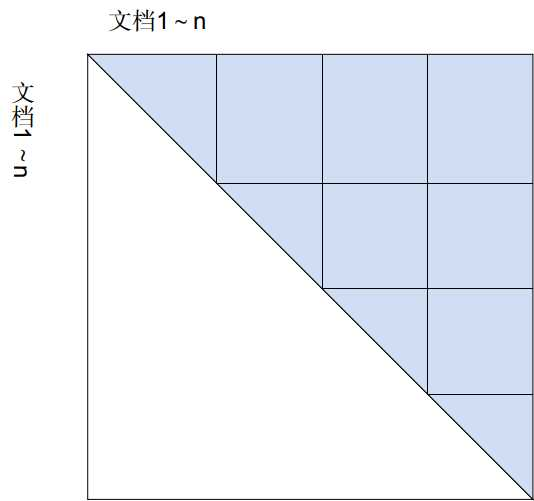
\includegraphics[width=0.35\textwidth]{triangle.jpg}
\end{figure}
\end{itemize}
\end{frame}
\begin{frame}{网页聚类模块介绍}
  \transdissolve<2->
  \begin{tikzpicture}[scale=.58,transform shape,
    font=\large,
    io/.style={fill=black!30, text width=3cm, minimum size=1cm,align=center,draw=black},
    submodule/.style={fill=cyan!80, text width=3cm, minimum size=1cm, rounded corners,align=center,draw=black},
    bold arrow/.style={very thick, >=triangle 90},
    mylabel/.style={dotted, draw}
    ]    
    \node (input) [io] {输入网页};
    \node (input-arrow) [below=1mm of input]
    [single arrow, minimum width=5mm, minimum height=0.8cm, shape border rotate=270, draw]{};
      \node (m1-1) [submodule, below=4mm of input-arrow]{过滤无用网页};
      \node (m1-2) [submodule, below=5mm of m1-1]{简化HTML文档} edge[<-] (m1-1);
    \node (m2-1) [submodule, below=1.2cm of m1-2]{结构相似度计算};
    \draw [<-, bold arrow] (m2-1) -- (m1-2);
    \visible<2->{\node (m2-2) [submodule, below=5mm of m2-1]{网页聚类} edge[<-] (m2-1);}
  \invisible<1->{
    \node (m3-1) [submodule, below=1.2cm of m2-2]{模板生成};
    \draw [<-, bold arrow] (m3-1) -- (m2-2);
    \node (m3-2) [submodule, below=5mm of m3-1]{内容抽取} edge[<-] (m3-1);
    \node (new-input) [io, left=of m3-2]{新的网页输入};
    \node (output) [io, below=of m3-2]{XML输出};
    \draw [->, bold arrow] (new-input) -- (m3-2);
    \draw [<-, bold arrow] (output) -- (m3-2);
    }
  \begin{pgfonlayer}{background}
    \tikzset{module/.style={inner sep=1em, fill=white, dashed, draw=black, rounded corners}};
    \node (m1)[module, fit=(m1-1) (m1-2)]{};
    \node (m1-name) [right=5mm of m1]{\Large{预处理模块}};
    \node (m2)[module, fit=(m2-1) (m2-2)]{} [below=of m1];
    \node (m2-name) [right=5mm of m2]{\Large{网页聚类模块}};
  \invisible<1->{
    \node (m3)[module, fit=(m3-1) (m3-2)]{} [below=of m2];
    \node (m37name) [right=5mm of m3] {\Large{模板生成和内容提取模块}};
  }
      \invisible<1->{
      \node (offline) [draw, inner sep=3mm, fill=orange!20, fit=(input) (m1-1) (m1-2) (m2-1) (m2-2) (m3-1)]
      [label={[red]right:\LARGE{离线处理部分}}]{};
      \node (online) [draw, inner sep=3mm, fill=green!30,fit=(m3-2) (new-input) (output), rounded corners]
      [label={[red]right:\LARGE{在线处理部分}}]{};}
  \end{pgfonlayer}  
\end{tikzpicture}
\end{frame}

\begin{frame}[label=sec-2-14]{聚类算法}
\begin{columns}
\begin{column}{0.4\textwidth}
\begin{enumerate}
\item 初始时,让每个文档实例都单独为一类
\item 迭代时,每次选择距离最近的两个类合并
\item 直到任意两个类的距离都大于阈值时程序退出
\item 算法的结束条件由阈值决定,无需实现设定类的个数。
\end{enumerate}

\end{column}

\begin{column}{0.6\textwidth}
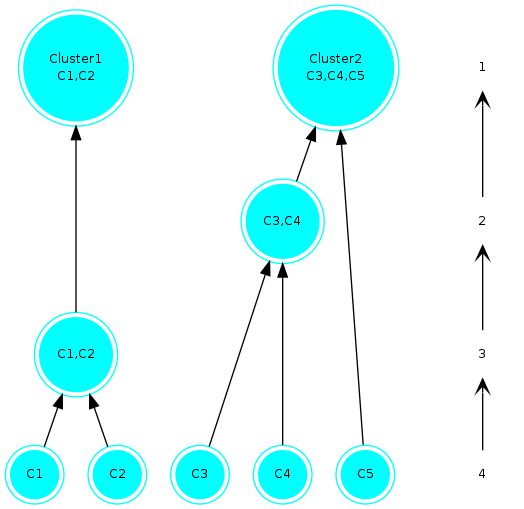
\includegraphics[width=\textwidth]{aggloclustering}

\end{column}
\end{columns}
\end{frame}

\subsection{模板生成和内容提取模块}

\begin{frame}{模板生成和内容提取模块介绍}
  \transdissolve<2->
  \begin{tikzpicture}[scale=.58,transform shape,
    font=\large,
    io/.style={fill=black!30, text width=3cm, minimum size=1cm,align=center,draw=black},
    submodule/.style={fill=cyan!80, text width=3cm, minimum size=1cm, rounded corners,align=center,draw=black},
    bold arrow/.style={very thick, >=triangle 90},
    mylabel/.style={dotted, draw}
    ]    
    \node (input) [io] {输入网页};
    \node (input-arrow) [below=1mm of input]
    [single arrow, minimum width=5mm, minimum height=0.8cm, shape border rotate=270, draw]{};
      \node (m1-1) [submodule, below=4mm of input-arrow]{过滤无用网页};
      \node (m1-2) [submodule, below=5mm of m1-1]{简化HTML文档} edge[<-] (m1-1);
    \node (m2-1) [submodule, below=1.2cm of m1-2]{结构相似度计算};
    \draw [<-, bold arrow] (m2-1) -- (m1-2);
     \node (m2-2) [submodule, below=5mm of m2-1]{网页聚类} edge[<-] (m2-1);
    \visible<4->{\node (m3-1) [submodule, below=1.2cm of m2-2]{模板生成};}
    \visible<2->{\draw [<-, bold arrow] (m3-1) -- (m2-2);}
  \invisible<1->{
    \node (m3-2) [submodule, below=5mm of m3-1]{内容抽取} edge[<-] (m3-1);
    \node (new-input) [io, left=of m3-2]{新的网页输入};
    \node (output) [io, below=of m3-2]{XML输出};
    \draw [->, bold arrow] (new-input) -- (m3-2);
    \draw [<-, bold arrow] (output) -- (m3-2);
    }
  \begin{pgfonlayer}{background}
    \tikzset{module/.style={inner sep=1em, fill=white, dashed, draw=black, rounded corners}};
    \node (m1)[module, fit=(m1-1) (m1-2)]{};
    \node (m1-name) [right=5mm of m1]{\Large{预处理模块}};
    \node (m2)[module, fit=(m2-1) (m2-2)]{} [below=of m1];
    \node (m2-name) [right=5mm of m2]{\Large{网页聚类模块}};
  \visible<3->{
    \node (m3)[module, fit=(m3-1) (m3-2)]{} [below=of m2];
    \node (m37name) [right=5mm of m3] {\Large{模板生成和内容提取模块}};
  }
      \invisible<1->{
      \node (offline) [draw, inner sep=3mm, fill=orange!20, fit=(input) (m1-1) (m1-2) (m2-1) (m2-2) (m3-1)]
      [label={[red]right:\LARGE{离线处理部分}}]{};
      \node (online) [draw, inner sep=3mm, fill=green!30,fit=(m3-2) (new-input) (output), rounded corners]
      [label={[red]right:\LARGE{在线处理部分}}]{};}
  \end{pgfonlayer}  
\end{tikzpicture}
\end{frame}

\begin{frame}[label=sec-2-15]{模板形式化定义}
\begin{block}{基本节点}
\begin{itemize}[<+->]
\item 两种组成方式 
\begin{enumerate}
\item 单个不重复的HTML标签,即 $<tag>$
\item 由一个或多个HTML标签组成的序列,这些序列可以出现一次或多次
\end{enumerate}
\item 第二种形式通过合并重复记录得到,对应的模板语言为:
\begin{figure}[hb]
\centering
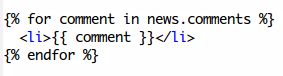
\includegraphics[width=0.4\textwidth]{django-for}
\end{figure}
\item 还有一种模板生成形式:
\begin{figure}[hb]
\centering
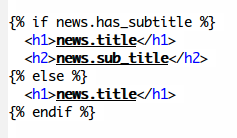
\includegraphics[width=0.35\textwidth]{django-if}
\end{figure}
\end{itemize}
\end{block}
\end{frame}
\begin{frame}[label=sec-2-16]{模板定义}
\begin{block}{必选和可选节点}
\begin{itemize}
\item 必选节点对应着由基本节点组成的一个序列
\item 可选节点同时对应多个序列,每个序列由不同的基本节点组成,同时每个序列
还对应着一个出现概率
\item 我们规定:模板$Tp$必须由必选节点$TN_i$和$ON_i$交替组成,第一个和最后一个可
  选节点是可选的:
      \[
      Tp=[ON_0]EN_1ON_1EN_2ON_2......EN_n[ON_n] 
      \]
\end{itemize}
\end{block}
\end{frame}

\begin{frame}[label=sec-2-17]{模板生成算法}
\begin{itemize}
\item 找出所有组成必选节点的基本节点:对于一个聚类的全部序列,从聚类中心点开始,
依次计算一次最长公共子序列,得到 $n$ 个序列的公共子序列 $S_{common}$
\item 每个序列和 $S_{common}$ 对齐,得到一些未对齐的区间,每个未对齐的区间计算一个
可选节点
\item 已对齐的基本节点组成必选节点
\item 必选节点和可选节点交替出现,组成最终的模板
\end{itemize}
\end{frame}

\begin{frame}[label=sec-2-18]{模板生成流程图}
  \vspace{-2mm}
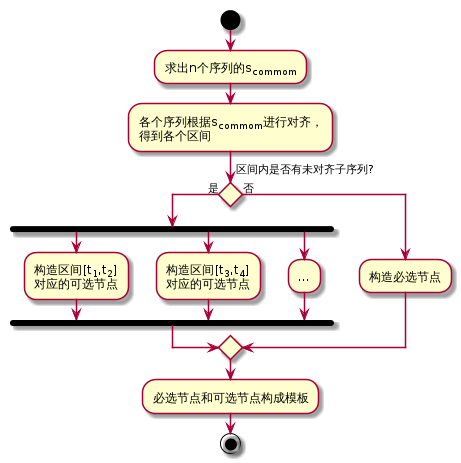
\includegraphics[width=0.8\textwidth]{subsystem}
\end{frame}

\begin{frame}[label=sec-2-19]{简单的例子}
\begin{itemize}
\item 设有3个序列,分别为:
\begin{eqnarray*}
s_1&=&aorzbcdlxe\\
s_2&=&athubeatcdlxe\\
s_3&=&athubeatcdpkue
\end{eqnarray*}
\item 根据最长公共子串算法,得到 $s_{common}$ 为 $abcde$
\item 每个序列同 $s_{common}$ 进行对齐,得到
\begin{displaymath}
\begin{matrix}
s_1      & : & \mathbf{a} & orz & \mathbf{b} &   & \mathbf{cd} &lx & \mathbf{e}\\
s_2      &:&\mathbf{a}&thu&\mathbf{b}&eat&\mathbf{cd}&lx&\mathbf{e}\\
s_3      &:&\mathbf{a}&thu&\mathbf{b}&eat&\mathbf{cd}&pku&\mathbf{e}\\
s_{common}&:&\mathbf{a}&   &\mathbf{b}&   &\mathbf{cd}&   &\mathbf{e}\\
\end{matrix}
\end{displaymath}
\end{itemize}
\end{frame}

\begin{frame}[label=sec-2-20]{简单的例子}
\begin{itemize}
\item 根据上述对齐结果,生成以下可选节点:
\begin{eqnarray*}
ON_{a,b}&=&(thu,2/3)~|~(orz,1/3)\\
ON_{b,c}&=&eat,2/3\\
ON_{d,e}&=&(lx,2/3)~|~(pku,1/3)
\end{eqnarray*}
\item 对齐的部分则对应生成必选节点,注意将连续的基本节点合并,分别为: $a,b,cd,e$
\end{itemize}
\end{frame}

\begin{frame}[label=sec-2-21]{可选节点生成的实际实现}
\begin{itemize}
\item 实际情况要比上面的例子复杂。区间 $[t_1,t_2]$ 中未对齐的那些标签子序列,有些可能差
异很大,有些则可能非常相近。
\item<2-> 做法:对于每个区间$[t_1,t_2]$,先将几种不同的子序列分开,然后针对每个子序列集合提取“模板”。
\item<3-> 我们发现,这和整体的框架很相似。因此,可选节点生成问题可以使用一个“自
  相似”的框架解决。
\end{itemize}
\end{frame}

\begin{frame}[label=sec-2-22]{构造可选节点流程}
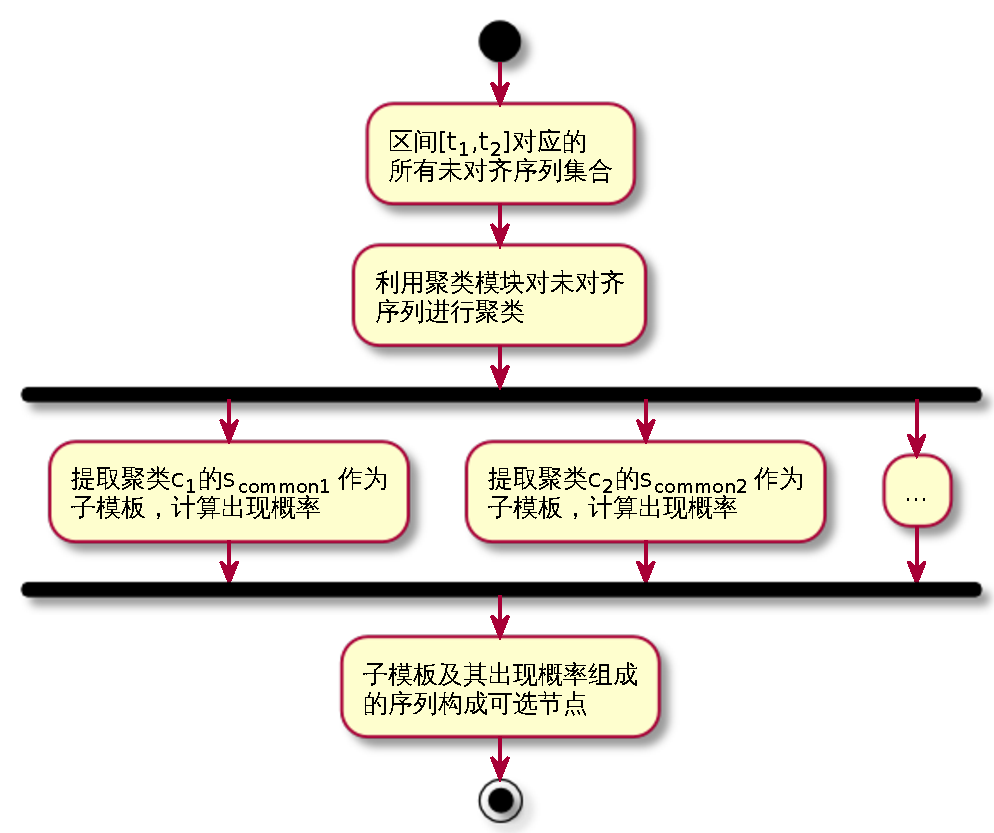
\includegraphics[width=0.9\textwidth]{subtemplate}
\end{frame}

\begin{frame}{模板生成和内容提取模块介绍}
  \transdissolve<2->
    \vspace{-2mm}
  \begin{tikzpicture}[scale=.57,transform shape,
    font=\large,
    io/.style={fill=black!30, text width=3cm, minimum size=1cm,align=center,draw=black},
    submodule/.style={fill=cyan!80, text width=3cm, minimum size=1cm, rounded corners,align=center,draw=black},
    bold arrow/.style={very thick, >=triangle 90},
    mylabel/.style={dotted, draw}
    ]    
    \node (input) [io] {输入网页};
    \node (input-arrow) [below=1mm of input]
    [single arrow, minimum width=5mm, minimum height=0.8cm, shape border rotate=270, draw]{};
      \node (m1-1) [submodule, below=4mm of input-arrow]{过滤无用网页};
      \node (m1-2) [submodule, below=5mm of m1-1]{简化HTML文档} edge[<-] (m1-1);
    \node (m2-1) [submodule, below=1.2cm of m1-2]{结构相似度计算};
    \draw [<-, bold arrow] (m2-1) -- (m1-2);
     \node (m2-2) [submodule, below=5mm of m2-1]{网页聚类} edge[<-] (m2-1);
    \node (m3-1) [submodule, below=1.2cm of m2-2]{模板生成};
    \draw [<-, bold arrow] (m3-1) -- (m2-2);
    \visible<3->{\node (m3-2) [submodule, below=5mm of m3-1]{内容抽取} edge[<-] (m3-1);}
    \visible<4->{\node (new-input) [io, left=of m3-2]{新的网页输入};}
    \visible<7->{\node (output) [io, below=of m3-2]{XML输出};}
    \visible<5->{\draw [->, bold arrow] (new-input) -- (m3-2);}
    \visible<6->{\draw [<-, bold arrow] (output) -- (m3-2);}
  \begin{pgfonlayer}{background}
    \tikzset{module/.style={inner sep=1em, fill=white, dashed, draw=black,
        rounded corners}};
    \invisible<2>{
    \node (m1)[module, fit=(m1-1) (m1-2)]{};
    \node (m1-name) [right=5mm of m1]{\Large{预处理模块}};
    \node (m2)[module, fit=(m2-1) (m2-2)]{} [below=of m1];
    \node (m2-name) [right=5mm of m2]{\Large{网页聚类模块}};
    \node (m3)[module, fit=(m3-1) (m3-2)]{} [below=of m2];
    \node (m37name) [right=5mm of m3] {\Large{模板生成和内容提取模块}};}
    \visible<2>{
      \node (offline) [draw, inner sep=3mm, fill=orange!20, fit=(input) (m1-1) (m1-2) (m2-1) (m2-2) (m3-1)]
      [label={[red]right:\LARGE{离线处理部分}}]{};}
      \visible<8->{
      \node (online) [draw, inner sep=3mm, fill=green!30,fit=(m3-2) (new-input) (output), rounded corners]
      [label={[red]right:\LARGE{在线处理部分}}]{};}
  \end{pgfonlayer}  
\end{tikzpicture}
\end{frame}

\begin{frame}[label=sec-2-23]{内容提取模块}
  \begin{columns}
    \begin{column}{0.4\textwidth}
      \begin{enumerate}[<+->]
  \item 人工标注感兴趣的内容,如新闻标题,正文等。
  \item 计算距离,判断使用哪个模板
  \item 与模板对齐,抽取内容
  \end{enumerate}
    \end{column}
    \begin{column}{0.6\textwidth}
\centering
    \vspace{-3mm}
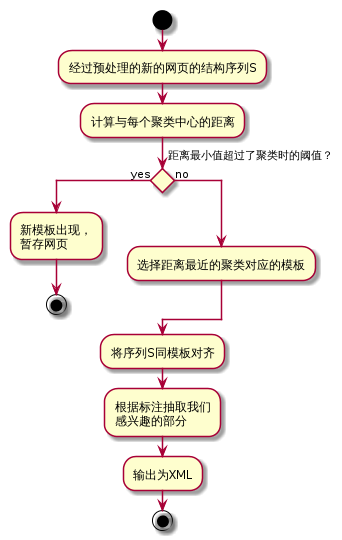
\includegraphics[width=\textwidth]{extractor}
    \end{column}
  \end{columns}
\end{frame}

\begin{frame}[label=sec-2-24]{模板匹配演示系统}
\begin{itemize}
\item 基于Play! Framework(Scala)实现了一个Web Service
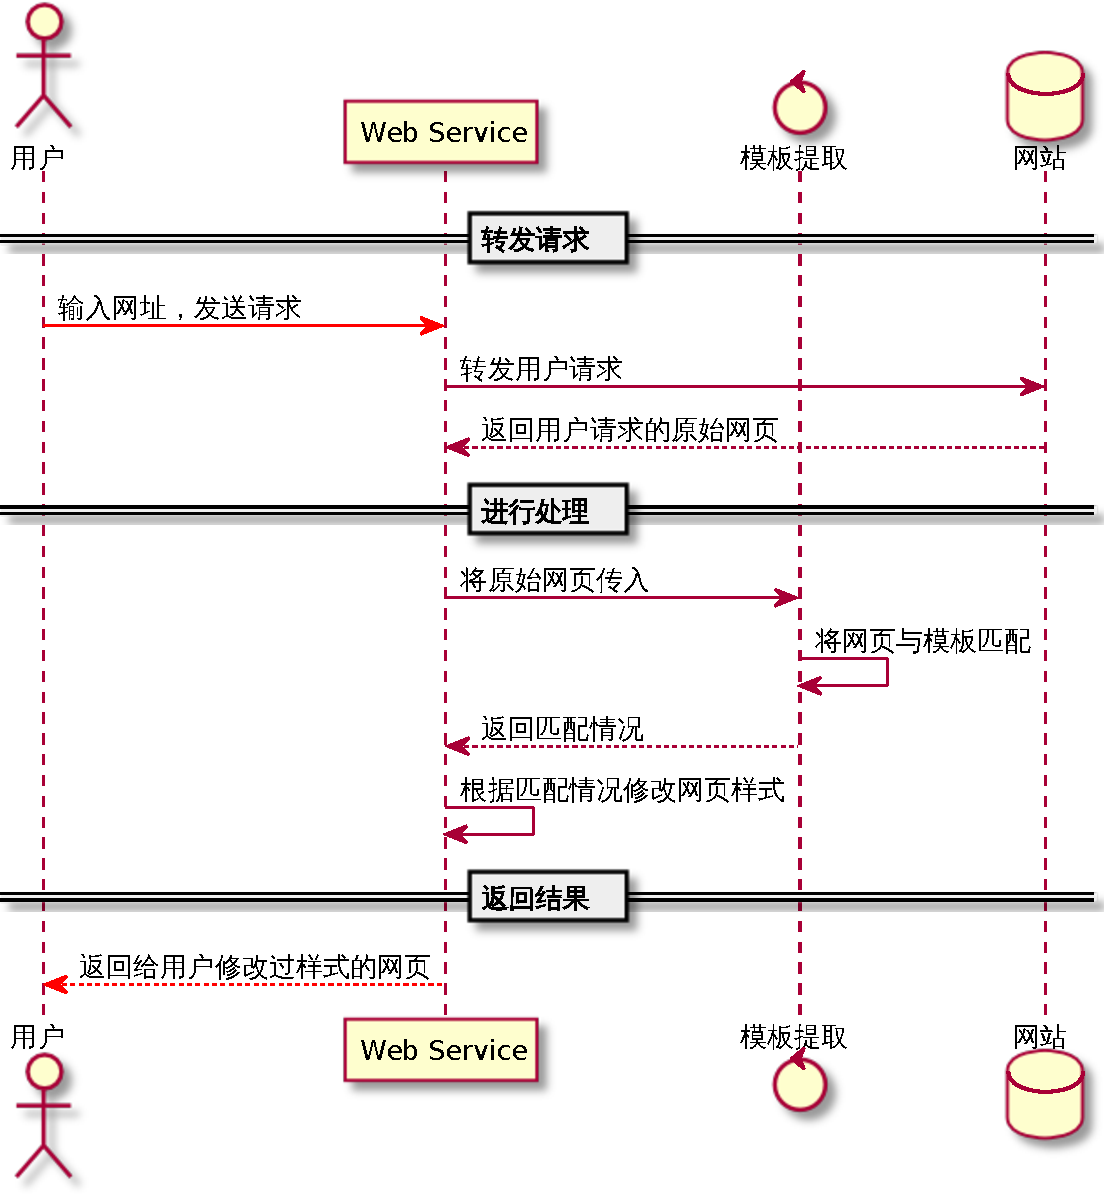
\includegraphics[width=0.6\textwidth]{demo}
\end{itemize}
\end{frame}

%%% Local Variables: 
%%% mode: latex
%%% TeX-master: "../final_report_beamer"
%%% End: 
